\documentclass{article}

% set font encoding for PDFLaTeX, XeLaTeX, or LuaTeX
\usepackage{ifxetex,ifluatex}
\if\ifxetex T\else\ifluatex T\else F\fi\fi T%
  \usepackage{fontspec}
\else
  \usepackage[T1]{fontenc}
  \usepackage[utf8]{inputenc}
  \usepackage{lmodern}
\fi

\usepackage{hyperref}

\title{Homework 1}
\author{Marshall Grimmett}

% Enable SageTeX to run SageMath code right inside this LaTeX file.
% http://doc.sagemath.org/html/en/tutorial/sagetex.html
% \usepackage{sagetex}

% Enable PythonTeX to run Python – https://ctan.org/pkg/pythontex
% \usepackage{pythontex}

\usepackage{amsmath}
\usepackage{pgfplots}
\pgfplotsset{compat=1.8}
\usepgfplotslibrary{statistics}

\usepackage{pgfplotstable}
\makeatletter
\long\def\ifnodedefined#1#2#3{%
    \@ifundefined{pgf@sh@ns@#1}{#3}{#2}%
}

\pgfplotsset{
    discontinuous/.style={
    scatter,
    scatter/@pre marker code/.code={
        \ifnodedefined{marker}{
            \pgfpointdiff{\pgfpointanchor{marker}{center}}%
             {\pgfpoint{0}{0}}%
             \ifdim\pgf@y>0pt
                \tikzset{options/.style={mark=*, fill=white}}
                \draw [densely dashed,blue] (marker-|0,0) -- (0,0);
                \draw plot [mark=*] coordinates {(marker-|0,0)};
             \else
                \tikzset{options/.style={mark=none}}
             \fi
        }{
            \tikzset{options/.style={mark=none}}
        }
        \coordinate (marker) at (0,0);
        \begin{scope}[options]
    },
    scatter/@post marker code/.code={\end{scope}}
    }
}

\makeatother

\begin{document}
\maketitle


\section{Part 1}


\subsection{a}

\begin{tikzpicture}
\begin{axis}[
    title={PMF},
    xlabel={Year in School},
    ylabel={Probability},
    xmin=.5, xmax=4.5,
    ymin=0, ymax=.4,
    xtick={1,2,3,4},
    ytick={},
    legend pos=north west,
    ymajorgrids=true,
    grid style=dashed,
]
\addplot[
    ycomb,
    color=blue,
    mark=square,
    ]
    coordinates {
    (1,1000/3186.625)(2,850/3186.625)(3,722.5/3186.625)(4,614.125/3186.625)
    };
    \legend{}
\end{axis}
\end{tikzpicture}

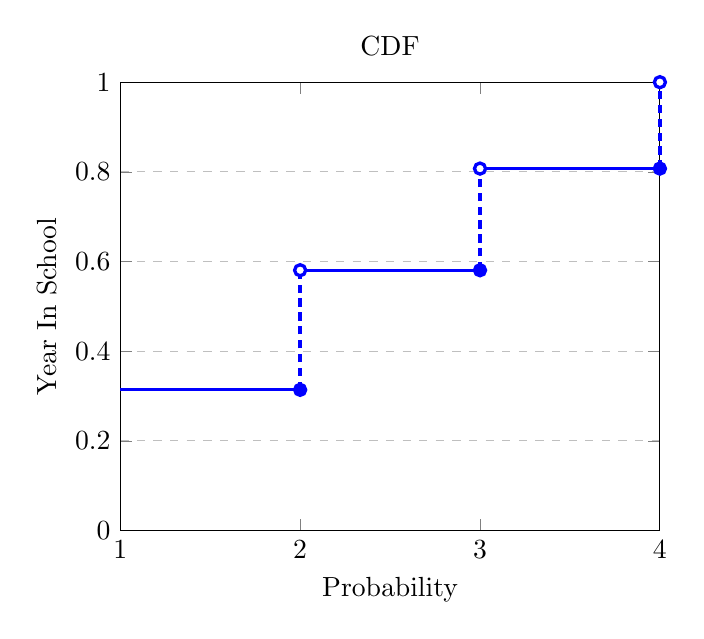
\begin{tikzpicture}
\begin{axis}[
    title={CDF},
    xlabel={Probability},
    ylabel={Year In School},
    xmin=1, xmax=4,
    ymin=0, ymax=1,
    xtick={1,2,3,4},
    ytick={},
    legend pos=north west,
    ymajorgrids=true,
    grid style=dashed,
    clip=false,
    jump mark left,
    every axis plot/.style={very thick},
    discontinuous,
    table/create on use/cumulative distribution/.style={
        create col/expr={\pgfmathaccuma + \thisrow{f(x)}}
    }
]
\addplot[
    color=blue,
    mark=square,
    ]
    coordinates {
    (1,1000/3186.625)(2,1850/3186.625)(3,2572.5/3186.625)(4,1)
    };
\end{axis}
\end{tikzpicture}

\subsection{b}
\begin{multline*}
\mu=\sum_{i=1}^{n}X_iP_i \\
=[(1*1000/3186.625)+(2*850/3186.625)\\
+(3*722.5/3186.625)+(4*614/3186.625)] \\
=2.2981995057466755
\end{multline*}

\begin{multline*}
\sigma^2=\frac{1}{n}\sum_{i=1}^{n}(X_i-\mu)^2 \\
=(1/3)*5.162893757923545 \\
=1.29072
\end{multline*}

\subsection{c}
\begin{equation*}
\mu=f(\alpha)=\sum_{i=1}^{n}\frac{X_i(1-\alpha)^{i-1}}{\sum_{i=0}^{n}\alpha^i}
\end{equation*}

\newpage

\subsection{d} Mean of University C

\begin{multline*}
\mu=(1*1000/3376.625)+(2*850/3376.625)+(3*722.5/3376.625) \\
+(4*614/3376.625)+(6*40/3376.625) \\
+(7*50/3376.625)+(8*100/3376.625) \\
=2.5805352978195684
\end{multline*}

The mean is not very sensitive to these new data points. The median stays at 2 for both Universities, so it is not at all sensitive to the new data. The mode stays at year 1 for both Universities.

\subsection{e}
The Median, Q1, and Q3 are all the same for both Universities. Therefore the box plots should be the exact same.
The only difference is the range.

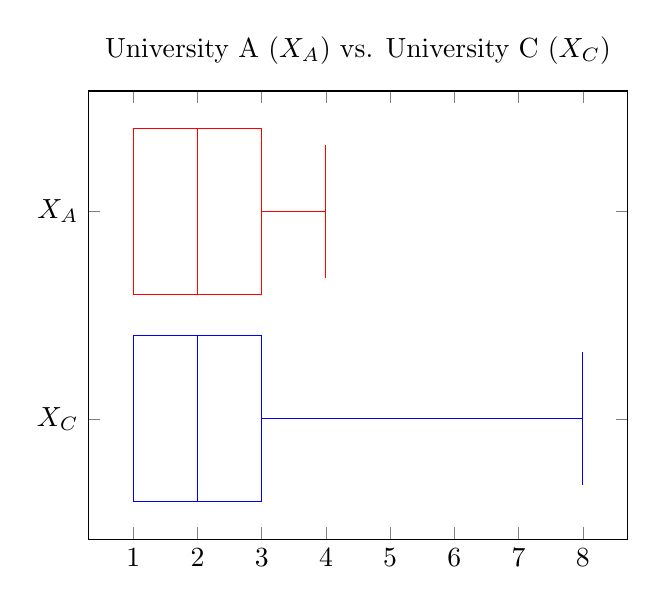
\begin{tikzpicture}
  \begin{axis}
    [
    title={University A ($X_A$) vs. University C ($X_C$)},
    xtick={1,2,3,4,5,6,7,8},
    ytick={1,2},
    yticklabels={$X_C$, $X_A$},
    ]
    \addplot+[
    boxplot prepared={
      median=2,
      upper quartile=3,
      lower quartile=1,
      upper whisker=8,
      lower whisker=1
    },
    ] coordinates {};
    \addplot+[
    boxplot prepared={
      median=2,
      upper quartile=3,
      lower quartile=1,
      upper whisker=4,
      lower whisker=1
    },
    ] coordinates {};
  \end{axis}
\end{tikzpicture}


\section{Part 2}


\subsection{a} PCA fails when the data appears non-linear, such as a circle or any other shape.
Another case would be if the data has no direction with significantly higher variance.

\subsection{b} A way to quantify this would be to look at the data from different directions to see if there are any non-linear shapes. We can also look at the principal components to see how much they differ.

\subsection{c}
In the below example, there is a plot of 8 data points that form a circle.
If we were to run PCA on this data and reduce it's dimension, this circle would be lost.
Also, we can see that along any new axis, there is hardly any change in variance. So if we projected horizontally it would be the same as projecting vertically.

\begin{tikzpicture}
\begin{axis}[
    title={Example Dataset},
    xlabel={X},
    ylabel={Y},
    xmin=0, xmax=5,
    ymin=0, ymax=5,
    xtick={0,1,2,3,4,5},
    ytick={0,1,2,3,4,5},
    legend pos=north west,
    ymajorgrids=true,
    grid style=dashed,
]
\addplot[
    only marks,
    scatter,
    color=blue,
    mark=square,
    ]
    coordinates {
    (1,2)(1,3)(2,4)(2,1)(3,1)(3,4)(4,2)(4,3)
    };
    \legend{}
\end{axis}
\end{tikzpicture}


\section{Part 3}

\subsection{a} See code.

\subsection{b}
Matrix Product: 0.0 second \\
Sum of Outer Products: 0.0050048828125 seconds \\
Sample Covariance: 0.4223923683166504 seconds \\

The Matrix product was the fastest and it happened so quickly that it recorded 0 seconds.
This is because computers can handle matrix multiplication very well and numpy can use smarter algorithms as well.For loops on the other hand, must happen sequentially so they cannot be optimized nearly as much as a single computation. The for loops are also have to perform a lot more computations. The sample covariance
was the slowest because it had to use 3 for loops resulting in $O(n^3)$ complexity.

\subsection{c} See code.

\subsection{d}
To compute $r$, I computed the fraction of total variance cumulatively for each component.
Once the threshold has been reached, the function exits with the value $r$.

\subsection{e}
\begin{figure}[h!]
  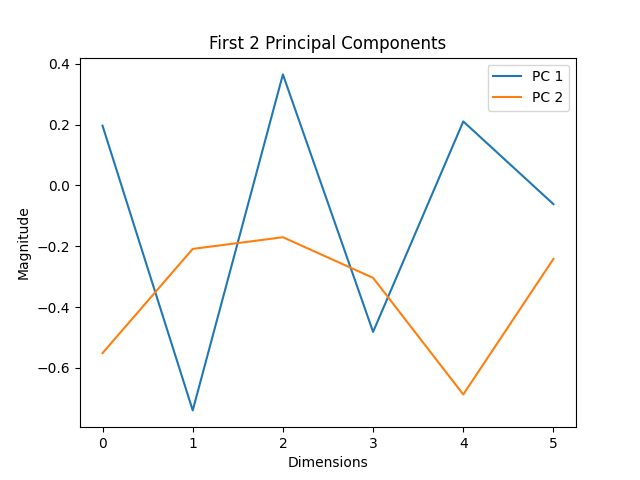
\includegraphics[width=\linewidth]{Figure_1.png}
\end{figure}

\subsection{f}
The reduced dimension data appears to have very high variance with one large centroid.
Smaller clusters can be picked out as well as some vacancies, but nothing significant.
The retained variance is $0.31759$. The top 2 principal components accounts for nearly $77\%$ of
the variance, while the top 3 account for $97\%$. While 3 components may be a better fit, 2 is still
very sufficient. Also, looking at the plot we can see a high degree of variation in the data. So, I would
say this is a good fit.


\end{document}
